\chapter{Vorarbeit}
\label{c:vorarbeit}


\section{Recherche zu Browser Extensions}
\label{s:recherchebrowserextensions}

\subsection{Extension-Programmierung allgemein}
\label{ss:extensionprogallg}

Unter einer Extension versteht man ein Programm, welches den Browser um neue Funktionen ergänzt. Durch eigene Oberflächen oder Manipulation der Website erleichtern diese Erweiterungen das Nutzen des Browser. 
Im Gegensatz zu Plug-Ins haben Extensions Zugriff auf Browser-spezielle Funktionen und sind in der Lage über die Webseite hinaus zu agieren. Plug-Ins werden direkt in eine Webseite eingebettet und sind auf diese beschränkt. Der Oberbegriff „Add-on“ wird heutzutage Hauptsächlich als Synonym für Extension verwendet.
Jeder größere Browser stellt eine Plattform zur Verfügung auf denen Extensions angeboten und installiert werden können. In der Regel sind Diese kostenlos. Können auch von außerhalb installiert werden zu Entwicklungszwecken oder wenn nicht auf der Plattform angeboten.
Extensions werden in HTML, JavaScript und CSS implementiert. Dabei können alle Bibliotheken verwendet werden, welche den Browserstandards für Extensions entsprechen. Kapitel 2.3.2 befasst sich genauer damit, welche Bedingungen für diese Bibliotheken in Google Chrome gelten.
Bekannte Beispiele sind Werbeblock wie UBlock Origin und VPN-Anwendungen wie Hola.

\subsection{Existieren bereits vergleichbare Extensions}
\label{ss:vergleichbareextensions}

Gesucht wurde nach einer Extension die auf der Play Store Seite den Nutzer datenschutzrelevante Informationen zu den angebotenen Apps liefert, Eine Datenschutzwertung im Playstore vergibt oder den Nutzer Apps nach Berechtigungen die Apps vorschlägt.
Extensions werden nach ihrer Kurzbeschreibung in den Suchergebnissen überprüft und bei nicht eindeutig Aufgabenbeschreibung die Infoseite aufgerufen(Bsp. Safe.ad im Web Store „ecosystem“).Nur deutsche und englische  Ergebnisse werden berücksichtigt.

Die Recherche hat ergeben, dass unter den genannten Suchkriterien keine Chrome oder Firefox Extension gefunden wurde die Aufgabenbereich der geplanten Extension abdeckt. Einige aufgeführte Beispiele implementieren einen Teil der geplanten Funktion (Umsortierung, Tracker checken) , aber keine Extension erfüllt alle gewünschten Aufgaben.


\subsection{Vergleich führender Browser als Plattform für die Extension}
\label{ss:vergleichbrowser}
Die getroffene Auswahl des Browsers als Plattform für die Entwicklung der Extension basiert hauptsächlich auf den aktuellen Marktanteilen. Google Chrome führt mit ca. 71\%, gefolgt von Mozilla Firefox mit 9,5\%, Microsoft Internet Explorer mit ca. 5,7\%, Apple Safari mit ca. 5\%, Microsoft Edge mit 4,4\% und Opera mit ca. 2,4\%.

\begin{figure}[ht]
	\centering
	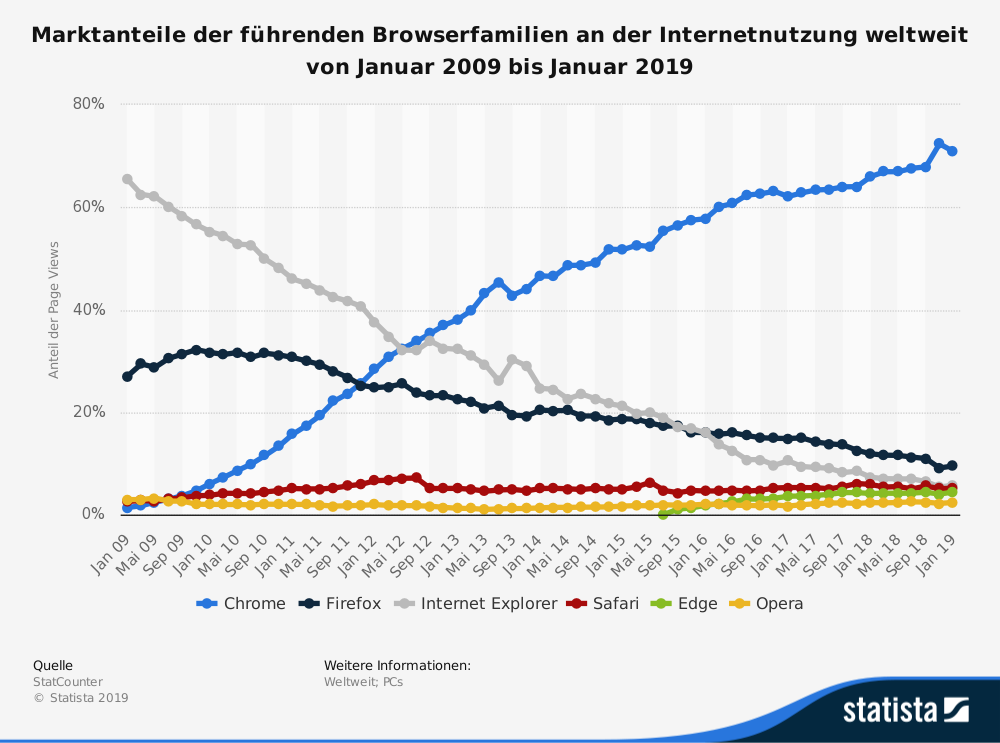
\includegraphics[width=1\textwidth]{pics/MarktanteileBrowser.png}
	\caption{StatCounter. n.d. Marktanteile der führenden Browserfamilien an der Internetnutzung weltweit von Januar 2009 bis Januar 2019. Statista. Zugriff am 4. März 2019. Verfügbar unter \url{https://de.statista.com/statistik/daten/studie/157944/umfrage/marktanteile-der-browser-bei-der-internetnutzung-weltweit-seit-2009/}.}
	\label{marktanteilebrowser}
\end{figure}
Aufgrund mangelnder Relevanz der Extension für Safari-Nutzer, sowie der Obsoleszenz des Internet Explorers, wurden diese Browser nicht weiter berücksichtigt.

Google Chrome ist den verbleibenden Alternativen Mozilla Firefox, Microsoft Edge und Opera im Punkt Marktanteile weit voraus und somit die gewählte Plattform zur Entwicklung der Extension.

Unabhängig der Implementierung bieten sowohl Mozilla\footnote{\url{https://developer.mozilla.org/en-US/docs/Mozilla/Add-ons/WebExtensions/Porting_a_Google_Chrome_extension}}, als auch Edge\footnote{\url{https://docs.microsoft.com/en-us/microsoft-edge/extensions/guides/porting-chrome-extensions}} eine intuitive Lösung zur Portierung der fertigen Google Chrome-Extension.

\section{PrivacyGuard}
\label{s:pguard}

\subsection{Vorstellung}
\label{ss:vorstellung}
Das Forschungsprojekt Privacy Guard\footnote{\url{https://datenschutz-scanner.de/das-projekt.html}} wurde im Januar 2016 durch das Bundesministerium für Bildung und Forschung ins Leben gerufen. Das Institut für Angewandte Informatik\footnote{\url{https://infai.org/}}, die mediaTest digital GmbH\footnote{\url{https://appvisory.com/company}}, die Quadriga Hochschule Berlin\footnote{\url{https://www.quadriga-hochschule.com/}} und die selbstregulierung informationswirtschaft e.V.\footnote{\url{https://sriw.de/}} haben gemeinsam Möglichkeiten entwickelt, Verbraucher auf die Verarbeitung ihrer Daten durch Handy-Applikationen aufmerksam zu machen. Dabei werden Vor- und Nachteile einzelner Aspekte der Datenverarbeitung erläutert und, bei Bedarf, Gegenmaßnahmen empfohlen.

\glqq Ziel [...] ist die Erleichterung des Selbstdatenschutzes für Verbraucher auf mobilen Endgeräten.\glqq{}(https://datenschutz-scanner.de/das-projekt.html,Stand 4.3.2019)

Die Ergebnisse des Projekts teilen sich in 3 Kategorien ein. Im Rahmen der Datenbeschaffung entstanden verschiedene Werkzeuge um Informationen über Apps zu extrahieren. Besonderer Wert wurde hier auf verlinkte Datenschutzerklärungen im Playstore und in der später installierten App auf dem Handy gelegt. Desweiteren wurden die Datenschutzerklärungen mittels eines entwickelten Pre-Tagging Tools, aber auch manuell annotiert, um die Verarbeitung der Texte zu optimieren.

Zur Datenverarbeitung entstand ein Backend\footnote{\url{https://pgadmin.datenschutz-scanner.de/api/docs.html}}, welches auf Anfrage der Bundle-ID einer App alle analysierten Daten übergibt. Dieses Backend bildet die Grundlage für die Datenvisualisierung von PGuard und ist die Schnittstelle der Informationen für die Browser-Extension.

Mit dem Projektabschluss im Juni 2018 stellte PrivacyGuard eine Webseite zur Analyse von Datenschutzerklärungen und Apps zur Verfügung\footnote{\url{https://dseanalyser.pguard-tools.de/}}. Als Prototypen entstanden zusätzlich eine App zur Analyse aller auf dem Handy installierten Applikationen auf ihren Datenschutz und die in dieser Arbeit behandelte Browser-Extension zur Visualisierung der, durch das Projekt gewonnenen, Informationen über Apps im PlayStore.

\subsection{API-Anbindung für die Extension}
\label{ss:apianbindung}

Sämtliche, von der Extension visualisierte, Daten werden über die Schnittstelle des Backends angefragt. Dazu benötigt die API mindestens eine Bundle-ID der App, Priorität und die Ausführtlichkeit der Antwort.

Je höher die Anfrage priorisiert ist, um so eher wird sie vom Backend verarbeitet. 
Bei einer hohen Ausführlichkeit umfassen die angeforderten Informationen komplette Datenschutzerklärungen und alle Metainformationen zur Datenbeschaffung. Dagegen beinhaltet eine Antwort mit niedriger Ausführlichkeit lediglich Sprache, Quelle und Extraktionsdatum der Datenschutzerklärung, sowie die Nummer der geltenden Infofelder mit jeweiligen Textpassagen aus der Datenschutzerklärung.

Für den Anwendungsfall der Browser-Extension besteht eine hohe Priorität um Wartezeiten möglichst gering zu halten. Dagegen reicht eine niedrige Ausführlichkeit zur Darstellung der nötigen Informationen für den Verbraucher. Zusätzlich bleibt so der Datenverkehr der Extension eher gering.

Die Infofelder sind der Hauptinformationsträger der Schnittstelle. Sie sind in 30 Eigenschaften unterteilt und können eine sogenannten "rote Linie" sein. Das bedeutet, dass bei Besitz dieser Eigenschaft, die entsprechende App potentiell gegen ein Gesetz verstößt. Folgenden Infofelder sind im Rahmen des PrivacyGuard Forschungsprojekts zur Beurteilung von Apps entstanden:
\begin{table}[h]
	\begin{tabular}{p{4.0cm}C{3.6cm}C{4.0cm}}
		\toprule
		\textbf{Property}		&	\textbf{Stereo Camera}		&	\textbf{Multi-Mode Radar \newline (near / far)}	\\
		\midrule
		meas. principle	&	CMOS sensor			&	FMCW			\\
		cycle time		&	60ms				&	66ms			\\
		latency			&	42ms				&	198ms			\\
		\midrule
		frequency		&	16fps				&	76 - 77 Ghz		\\
		bandwidth		&	---					&	187 Mhz			\\
		\midrule
		opening angle	&	45°					&	60° / 18°			\\
		range			&	500m \newline (3D-vision: 50m)	&	~60m	/ 200m		\\
		\midrule
		angle accuracy ($3\sigma$)		&	---	&	~~$\pm$ 1° / $\pm$ 0.1°		\\
		distance accuracy ($3\sigma$)	&	---	&	$\pm$ 0.25m		\\
		velocity accuracy ($3\sigma$)	&	---	&	$\pm 0.278 \tfrac{m}{s}$ / $\pm 0.139 \tfrac{m}{s}$	\\
		\bottomrule
	\end{tabular}
	\caption{Overview of the properties of several sensors}
	\label{tab:sensor_properties}
\end{table}

\section{Implementierung einer Google Chrome Extension}
\label{s:implementierung}
 stsa
\subsection{Eigenschaften}
\label{ss:eigenschaften}

Die Architektur einer Chrome Extension stellt ein Paket aus mehreren Dateien dar und ist vergleichbar mit anderen Web-Technologien wie zum Beispiel Webseiten.
Grundvoraussetzung für eine funktionierende Extension ist die manifest.json, welche grundlegende Informationen für den Browser bereitstellt und festlegt mit welchen Dateien und Rechten die Extension aufgebaut ist. Hinzu kommt mindestens eine HTML-Datei zur Darstellung der Inhalte und mindestens ein Skript zur Umsetzung der Funktionalität. Erweitert werden diese oft durch CSS-Dateien.
Externe Bibliotheken wie JQuery können ebenfalls eingebunden werden, müssen aber aufgrund der Policies von Google Chrome vollumfänglich lokal vorliegen. Mehr dazu Im nächsten Abschnitt.
Die Manifest-Datei ist im JSON-Format aufgebaut und beinhaltet sämtliche Informationen über die Extension. Wichtige Punkte sind Name der Extension, Beschreibung, Rechte und Aufbau. Unter Rechten oder „permissions“ werden alle APIs aufgelistet, welche die Extension benötigt um ordnungsgemäß zu funktionieren. Bevor ein Nutzer später die Extension installiert, muss er diesen „permissions“ zustimmen. Mehr zu den APIs im entsprechenden Abschnitt.
Der Aufbau wird unter „content scripts“ (BILD?) in drei Eigenschaften unterteilt: unter welchem URL sind die Skripte aktiv, welche Skripte sind dort aktiv und welche CSS-Dateien werden dort von der Extension eingesetzt.
HTML-Dateien werden als „User-Interface Elemente“ zusammengefasst und beinhalten im Normalfall eine popup.html zur Darstellung des Fensters der Extension in der oberen rechten Ecke des Browser-Fensters (BILD?). Je nach Funktionsumfang können weitere UI-Elemente eingebunden sein, um zum Beispiel die besuchte Webseite zu erweitern.

Die vorhandenen Skripte werden normalerweise in zwei Kategorien eingeteilt. Das sogenannte „Background-Skript“ dient als Event-Handler und kommuniziert zwischen Extension und Browser. Alle restlichen Skripte sind „Content-Skripte“. Sie beinhalten die eigentliche Funktionalität der Extension. 

\subsection{Funktionsumfang}
\label{ss:funktionsumfang}

\subsection{Darstellung im Browser}
\label{ss:darstellung}


\section{Caching-Methoden}
\label{s:cachingmethoden}

\subsection{Welche Rolle spielt Performance?}
\label{ss:rolleperformance}

\subsection{Verwendete Methoden und deren Eigenschaften}
\label{ss:methodeneigenschaften}



















